% Exam Template for UMTYMP and Math Department courses
%
% Using Philip Hirschhorn's exam.cls: http://www-math.mit.edu/~psh/#ExamCls
%
% run pdflatex on a finished exam at least three times to do the grading table on front page.
%
%%%%%%%%%%%%%%%%%%%%%%%%%%%%%%%%%%%%%%%%%%%%%%%%%%%%%%%%%%%%%%%%%%%%%%%%%%%%%%%%%%%%%%%%%%%%%%

% These lines can probably stay unchanged, although you can remove the last
% two packages if you're not making pictures with tikz.
\documentclass[11pt]{exam}
\RequirePackage{amssymb, amsfonts, amsmath, latexsym, verbatim, xspace, setspace}
\RequirePackage{tikz, pgflibraryplotmarks}

% By default LaTeX uses large margins.  This doesn't work well on exams; problems
% end up in the "middle" of the page, reducing the amount of space for students
% to work on them.
\usepackage[margin=1in]{geometry}
\usepackage{enumerate}
\usepackage{amsthm}

\theoremstyle{definition}
\newtheorem{soln}{Solution}

% Here's where you edit the Class, Exam, Date, etc.
\newcommand{\class}{Math 150A Section 8,16}
\newcommand{\term}{Fall 2025}
\newcommand{\examnum}{Exam I}
\newcommand{\examdate}{February 13, 2025}
\newcommand{\timelimit}{1 Hour 50 Minutes}

% For an exam, single spacing is most appropriate
\singlespacing
% \onehalfspacing
% \doublespacing

% For an exam, we generally want to turn off paragraph indentation
\parindent 0ex

\begin{document} 

% These commands set up the running header on the top of the exam pages
\pagestyle{head}
\firstpageheader{}{}{}
\runningheader{\class}{\examnum\ - Page \thepage\ of \numpages}{\examdate}
\runningheadrule

\begin{flushright}
\begin{tabular}{p{2.8in} r l}
\textbf{\class} & \textbf{Name (Print):} & \makebox[2in]{\hrulefill}\\
\textbf{\term} &&\\
\textbf{\examnum} & \textbf{Student ID:}&\makebox[2in]{\hrulefill}\\
\textbf{\examdate} &&\\
\textbf{Time Limit: \timelimit} % & Teaching Assistant & \makebox[2in]{\hrulefill}
\end{tabular}\\
\end{flushright}
\rule[1ex]{\textwidth}{.1pt}


This exam contains \numpages\ pages (including this cover page) and
\numquestions\ problems.  Check to see if any pages are missing.  Enter
all requested information on the top of this page, and put your initials
on the top of every page, in case the pages become separated.\\

You may \textit{not} use your books or notes on this exam.  However, you may use a \textit{basic} calculator.\\

You are required to show your work on each problem on this exam, unless otherwise stated.
The following rules apply:\\

\begin{minipage}[t]{3.7in}
\vspace{0pt}
\begin{itemize}

%\item \textbf{If you use a ``fundamental theorem'' you must indicate this} and explain
%why the theorem may be applied.

\item \textbf{Organize your work}, in a reasonably neat and coherent way, in
the space provided. Work scattered all over the page without a clear ordering will 
receive very little credit.  

\item \textbf{Mysterious or unsupported answers will not receive full
credit}.  A correct answer, unsupported by calculations, explanation,
or algebraic work will receive no credit; an incorrect answer supported
by substantially correct calculations and explanations might still receive
partial credit.  This especially applies to limit calculations.

\item If you need more space, use the back of the pages; clearly indicate when you have done this.

\item \textbf{Box Your Answer} where appropriate, in order to clearly indicate what you consider the answer to the question to be.

\item Unless otherwise stated, all angles are in \textbf{radians}
\end{itemize}

Do not write in the table to the right.
\end{minipage}
\hfill
\begin{minipage}[t]{2.3in}
\vspace{0pt}
%\cellwidth{3em}
\gradetablestretch{2}
\vqword{Problem}
\addpoints % required here by exam.cls, even though questions haven't started yet.	
\gradetable[v]%[pages]  % Use [pages] to have grading table by page instead of question

\end{minipage}
\newpage % End of cover page

%%%%%%%%%%%%%%%%%%%%%%%%%%%%%%%%%%%%%%%%%%%%%%%%%%%%%%%%%%%%%%%%%%%%%%%%%%%%%%%%%%%%%
%
% See http://www-math.mit.edu/~psh/#ExamCls for full documentation, but the questions
% below give an idea of how to write questions [with parts] and have the points
% tracked automatically on the cover page.
%
%
%%%%%%%%%%%%%%%%%%%%%%%%%%%%%%%%%%%%%%%%%%%%%%%%%%%%%%%%%%%%%%%%%%%%%%%%%%%%%%%%%%%%%

\begin{questions}

\addpoints

\question[10]\mbox{}
\textbf{TRUE or FALSE!}
If the statement is true, write TRUE (all caps, all spelled out).
Otherwise write FALSE (all caps, all spelled out).
\begin{enumerate}[(a)]
\item the function $\sin(x^2)$ is even
\vspace{1.2in}
\item the limit $\lim_{x\rightarrow\infty} f(x)$ is always either $0$ or $\infty$
\vspace{1.2in}
\item $(f(x)/g(x))' = f'(x)/g'(x)$
\vspace{1.2in}
\item a rational function is continuous at every point in its domain
\vspace{1.2in}
\item if $f(x)$ has a discontinuity at $3$, then $f'(3)$ does not exist
\end{enumerate}

\newpage
\question[10]\mbox{}
Calculate the following.  Carefully show you work.
\begin{enumerate}[(a)]
\item $\lim_{x\rightarrow 3}\frac{x^2+3x-18}{x-3}$
\vspace{2in}
\item $\lim_{x\rightarrow 2}\frac{\sqrt{x+2}-\sqrt{2x}}{x-2}$
\vspace{2in}
\item $\lim_{x\rightarrow 1}\frac{\frac{x+1}{x}-\frac{2}{x}}{x-1}$
\vspace{2in}
\item $\lim_{x\rightarrow \infty}\sqrt{x^2+x}-x$
\vspace{2in}
\end{enumerate}

\newpage
\question[10]
Draw a graph of the derivative of the function $f(x)$ whose graph is given below.
Carefully label the $x$ and $y$ axes and also indicate any points where the derivative does not exist.
\vspace{0.5in}
\begin{center}
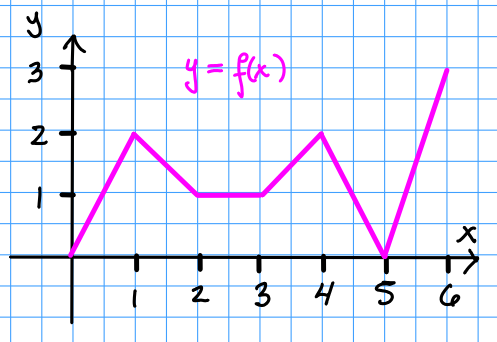
\includegraphics[width=.7\linewidth]{img/fig1.png}
\end{center}

\newpage
\question[10]\mbox{}
In lectures, we went over many important examples.
For each of the following, give an explicit example.
You do not need to show any work.
\begin{enumerate}[(a)]
\item  An odd function.
\vspace{1.5in}
\item  A limit which does not exist
\vspace{1.5in}
\item  A function with a jump discontininuity.
\vspace{1.5in}
\item  A function with a vertical asymptote at $x=2$
\vspace{1.5in}
\item  A function which is continuous at $0$ but which is not differentiable at $0$.
\vspace{1.5in}
\end{enumerate}


\newpage
\question[10]
\begin{enumerate}[(a)]
\item Carefully write down the $\epsilon$,$\delta$-definition of a limit.
\vspace{2in}
\item Let $f(x) = 1/x$.  For what range of $x$-values do we have $|f(x)-1| < 0.01$?
\end{enumerate}

\newpage
\question[10]
Calculate the derivative of each of the following functions.
\begin{enumerate}[(a)]
\item $f(x) = x^3 + \sin(x)$
\vspace{2in}
\item $g(t) = \frac{\sqrt{t} + t^2}{t}$
\vspace{3in}
\item $q(s) = \frac{(s^2+s^3)^2}{s^{-3}}$
\end{enumerate}

\newpage
\question[10]\mbox{}
Consider functions $f(x)$, $g(x)$, and $h(x)$ whose values satisfy
\begin{center}
\begin{tabular}{c|c|c|c|c|c|c|c}
$x$ & 1 & 2 & 3 & 4 & 5 & 6 & 7\\\hline
$f(x)$ & 1 & 1 & 2 & 3 & 5 & 8 & 13\\\hline
$f'(x)$ & 0 & 1 & 3 & 2 & 7 & 9 & 4\\\hline
\end{tabular}\\
\vspace{0.3in}
\begin{tabular}{c|c|c|c|c|c|c|c}
$x$ & 1 & 2 & 3 & 4 & 5 & 6 & 7\\\hline
$g(x)$ & 8 & 6 & 7 & 5 & 3 & 0 & 9\\\hline
$g'(x)$ & 0 & 1 & 0 & 1 & 2 & 3 & 5
\end{tabular}\\
\vspace{0.3in}
\begin{tabular}{c|c|c|c|c|c|c|c}
$x$ & 1 & 2 & 3 & 4 & 5 & 6 & 7\\\hline
$h(x)$ & 2 & 3 & 5 & 7 & 1 & 13 & 17\\\hline
$h'(x)$ & 4 & 3 & 2 & 1 & 2 & 3 & 4
\end{tabular}
\end{center}
Evaluate the following expressions.
\begin{enumerate}[(a)]
\item $F(5)$ for $F(x) = f(x) + 2g(x) - h(x)$
\vspace{1in}
\item $F'(5)$ for $F(x) = f(x) + 2g(x) - h(x)$
\vspace{1in}
\item $F(2)$ for $F(x) = g(f(4))) + f(g(4))$
\vspace{1in}
\item $F'(3)$ for $F(x) = x^3 + 7x + g(x)$
\end{enumerate}
\newpage
\question[10]\mbox{}
\begin{enumerate}[(a)]
\item Write down the formal definition of the derivative $f'(x)$ of $f(x)$.
\vspace{2in}
\item Using \textbf{only} the formal definition of a derivative and any limit laws, calculate $f'(x)$ for
$$f(x) = \frac{1}{\sqrt{2x+3}}.$$
\end{enumerate}
\end{questions}
\end{document}

